\documentclass[11pt,english,a4paper,twoside]{article}
%\documentclass[11pt,slovak,a4paper,twoside]{article}

\usepackage[IL2]{fontenc}
\usepackage[utf8]{inputenc}
\usepackage{babel}
\usepackage{url}
\usepackage[nottoc]{tocbibind}
\usepackage{ifthen}
\usepackage[hidelinks]{hyperref}
\usepackage{graphicx}
\usepackage{listings}
\usepackage{float}

\raggedbottom
\oddsidemargin=0cm
\evensidemargin=0cm
\textwidth=16.5cm
\pagestyle{plain}

\newcommand{\reporttitle}{AASS Semestral project}

\title{\reporttitle}

\author{
        Lukáš Častven, Michal Kilian\\[2pt]
	{\small Slovenská technická univerzita v Bratislave}\\
	{\small Fakulta informatiky a informačných technológií}\\
	{\small \texttt{xcastven@stuba.sk, xkilian@stuba.sk}}
}

\date{\today}
\begin{document}
\maketitle

\section{Application overview}

Our application is a simple medical calendar in which a patient can request and appointment,
doctor can accept it or deny it as well as add resources such as specialized medical facility,
medicine, or equipment. In this calendar patient can also see his/her medical conditions and
prescriptions history.

\section{Stakeholders}

\begin{table}[h!]
  \centering
  \begin{tabular}{|p{0.25\linewidth}|p{0.5\linewidth}|}
    \hline
    \textbf{Stakeholder} & \textbf{Description} \\
    \hline
    Patient & Wants to book appointment with doctor. \\
    \hline
    Medical staff & Accepts or rejects appointment requests,
    and selects specialized facilities, equipment or medicine. \\
    \hline
    Other hospital staff & Needs to see the availability of
    other doctors and specialized rooms for their patients. \\
    \hline
    Hospital & Desires a new application to organize
    doctors and appointments. \\
    \hline
  \end{tabular}
  \caption{Stakeholders and their descriptions}
  \label{tab:stakeholders}
\end{table}

\section{Motivation}

The following motivation diagram contains the drivers, assessments, goals,
outcomes, and requirements related to the 3 identified stakeholders.
Patient, Hospital, Nurse, Doctor.

The core problems, "High operational costs", "Long waiting times", and a "Bad
reputation for possible new hires", drive the hospital for change. These drivers
are associated with issues such as "Ineffective allocation", "Medical
staff frustration", "Unavailability of specialized rooms",
and patients' "Waiting times."

\pagebreak
\begin{figure}[ht]
    \centering
    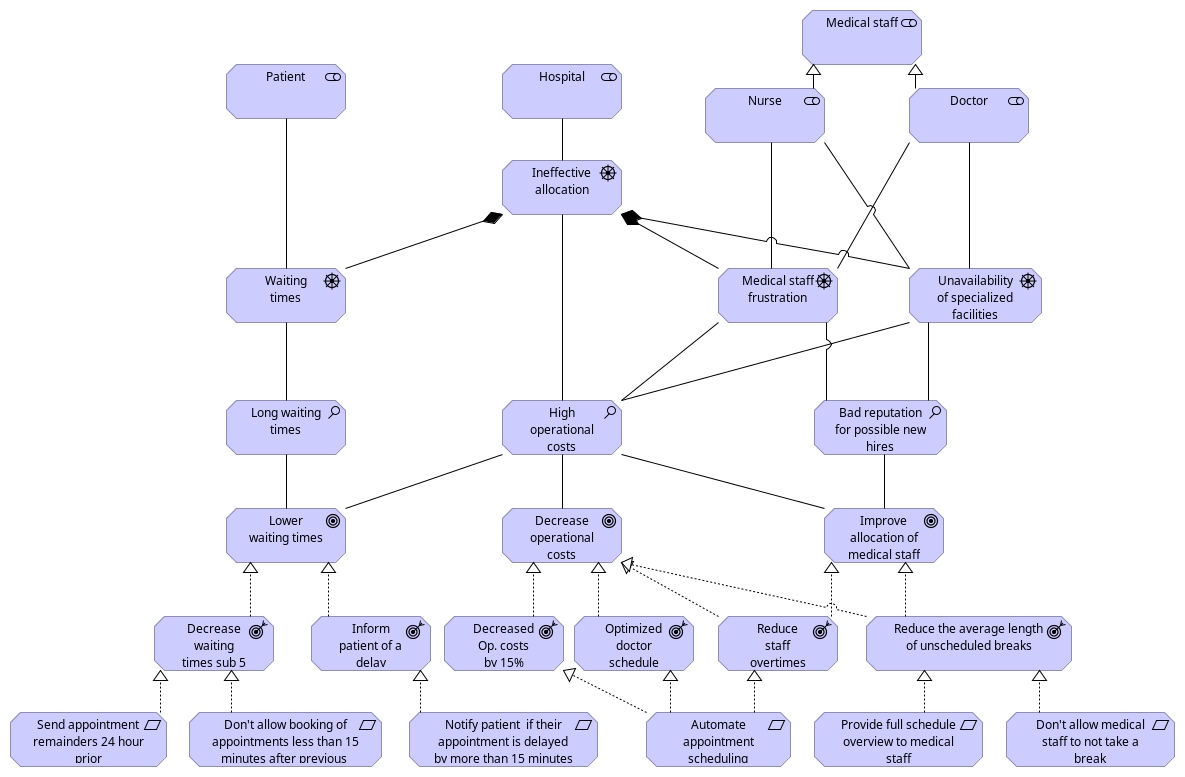
\includegraphics[width=\textwidth]{./fig/general/1. Motivation.png}
    \caption{Motivation layer}
    \label{fig:motivation}
\end{figure}

\pagebreak
\section{Value stream}

The value stream of scheduling an appointment realizes the outcome of optimized
doctor schedule.

\begin{figure}[ht]
    \centering
    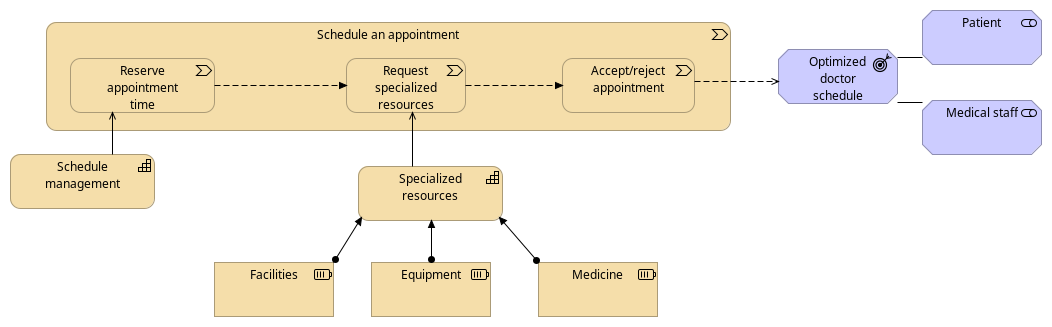
\includegraphics[width=\textwidth]{./fig/general/2. Value stream.png}
    \caption{Value stream: Scheduling appointment}
    \label{fig:value_stream}
\end{figure}

\pagebreak
\section{Business layer}

Following diagram models three business processes, which serve the patient
and medical staff to manage schedule.

\begin{figure}[ht]
    \centering
    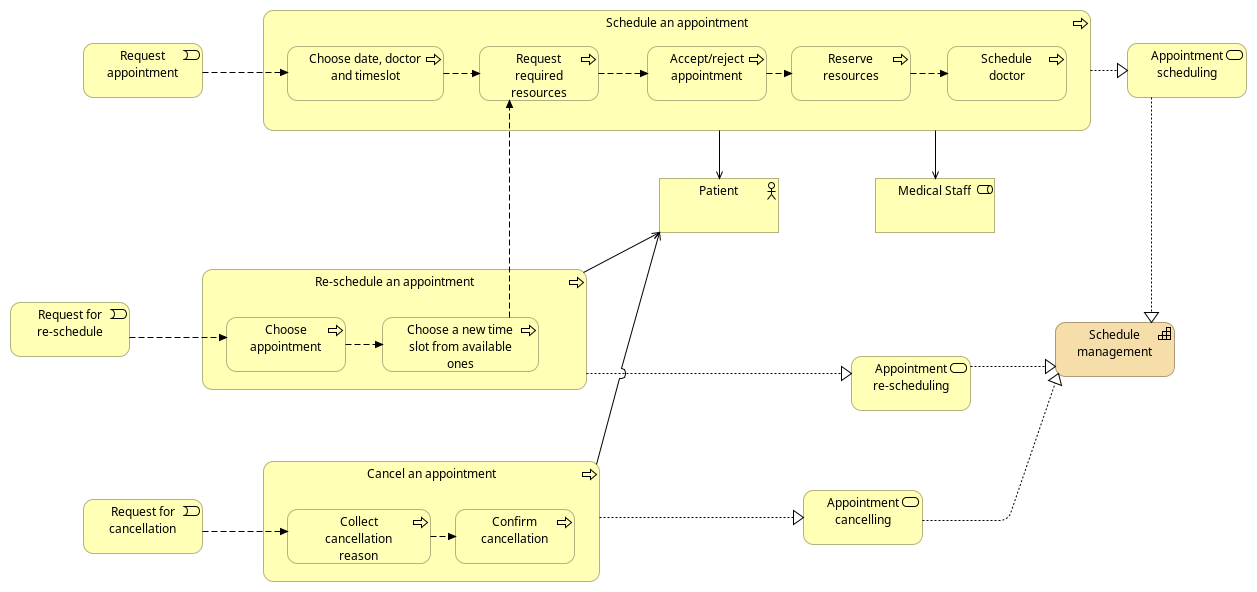
\includegraphics[width=\textwidth]{./fig/general/3. Business.png}
    \caption{Business layer}
    \label{fig:business}
\end{figure}

% TODO kili, this is the end of overview of the application and now write about the implementation
% use the ./fig/1. Business Implementation.png and describe only that process will be implemented

\section{Mockups}

The patient interface, Figure~\ref{fig:patient-mockups}, shows
a design centered on appointment scheduling.
Figure~\ref{fig:medical-staff-mockups} illustrates the UI for the
same use case, but with more control and additional resources requested
by the medical staff.

\begin{figure}[H]
    \centering
    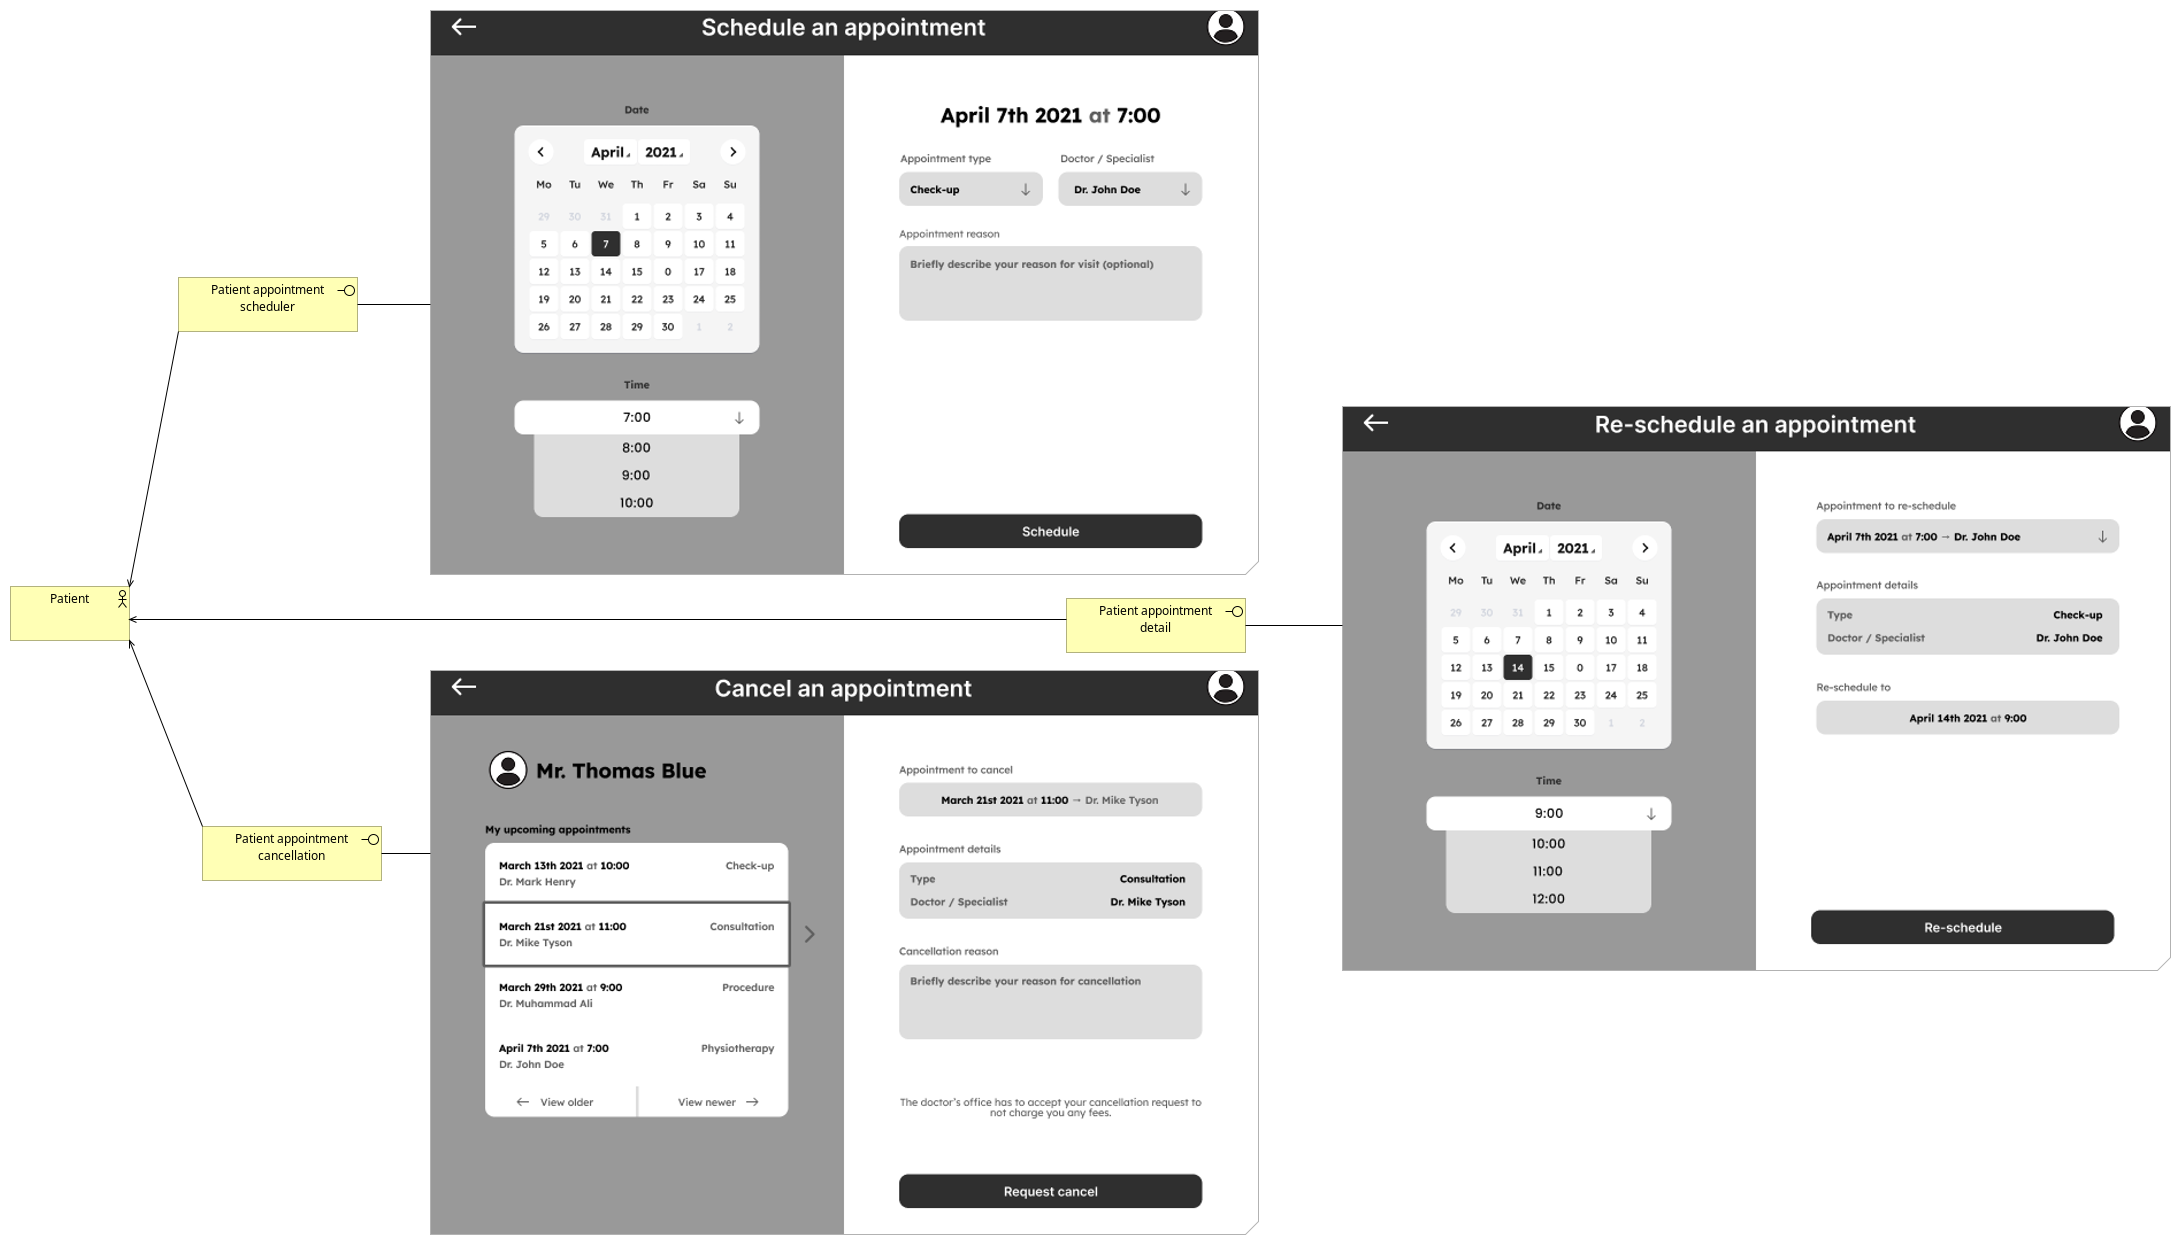
\includegraphics[width=\textwidth]{./fig/2. Business Frontend Patient.png}
    \caption{Patient's UI mockups}
    \label{fig:patient-mockups}
\end{figure}

\begin{figure}[H]
    \centering
    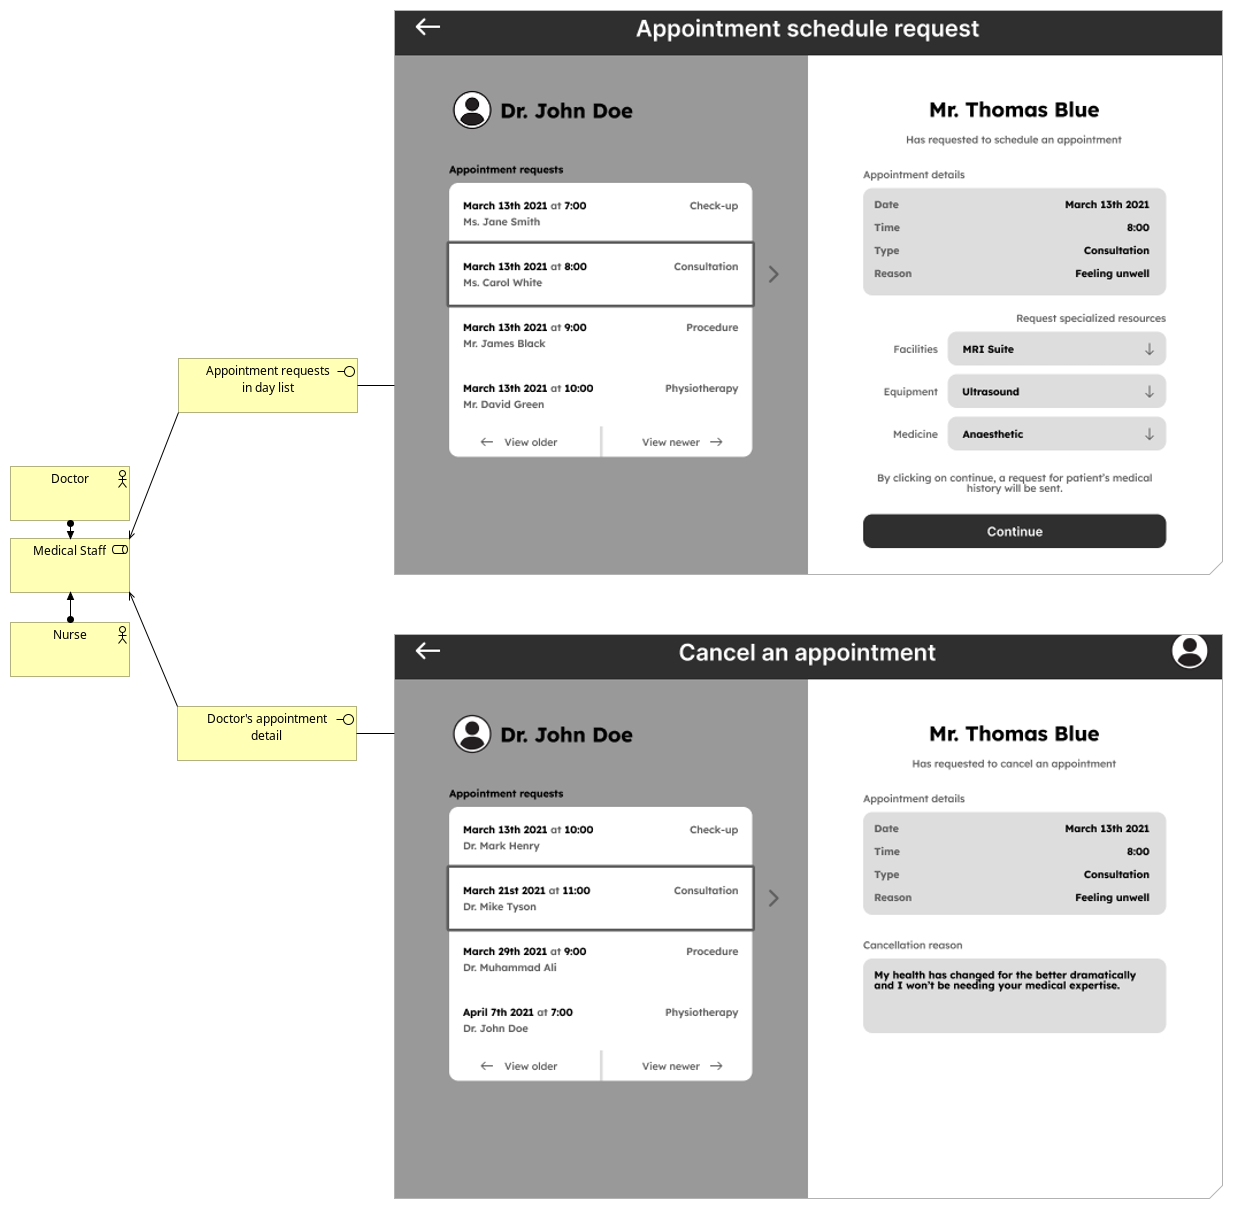
\includegraphics[width=\textwidth]{./fig/3. Business Frontend Medical staff.png}
    \caption{Medical staff's UI mockups}
    \label{fig:medical-staff-mockups}
\end{figure}

\section{Architecture}

We will implement a user interface and a back-end components to
support the "Schedule an appointment" business process.

\begin{figure}[H]
    \centering
    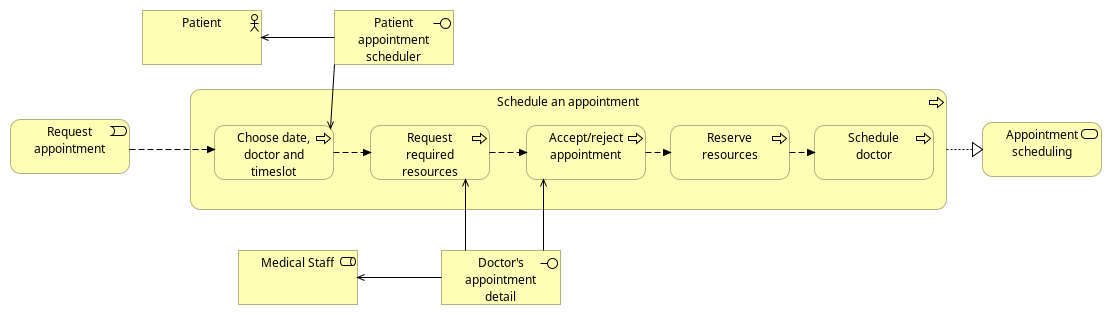
\includegraphics[width=\textwidth]{./fig/1. Business Implementation.png}
    \caption{Schedule an appointment process implementation}
    \label{fig:business-application}
\end{figure}

The implementation
will consist of a web application front-end developed using Stencil.js,
and back-end written in 4 different architectures:

\begin{enumerate}
    \item A monolithic backend
    \item Microservices
    \item Camunda oriented architecture
    \item Event driven architecture with Kafka
\end{enumerate}

The frontend implementation of the web app doesn't have to change/adapt
to the different architectures and is written once.

How the web application is connected to the mock-ups and the process as a whole is
shown in Figure~\ref{fig:business-application}. Both types of users access the core functionality of appointment scheduling through the Web app. The diagram further details that Medical Staff interact specifically with the "Doctor's appointment detail", while Patients utilize the "Patient appointment scheduler" interface within the Web app.

\begin{figure}[H]
    \centering
    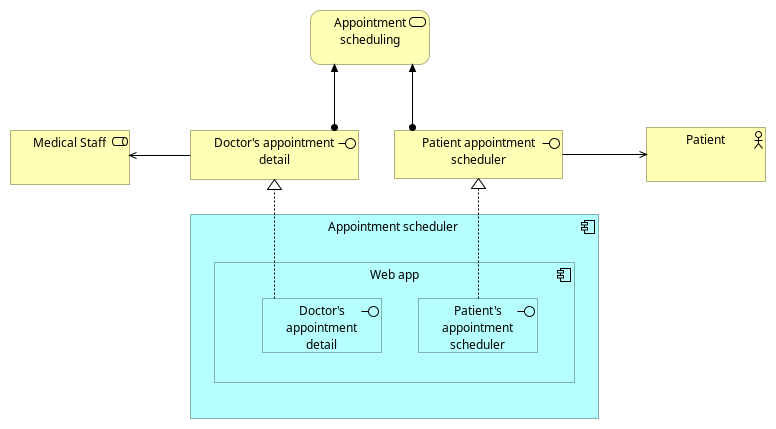
\includegraphics[width=\textwidth]{./fig/4. Business Application.png}
    \caption{Business Application}
    \label{fig:business-application}
\end{figure}

\subsection{A monolithic backend}

As for the first implementation, Figure~\ref{fig:monolith} details the
internal structure and data dependencies of the core "Appointment scheduler"
component. This component interacts with several data objects
including "Users" (specialized into "Patients" and "Doctors"), "Free
timeslots", "Appointments", and "Resources" (which are further categorized
into "Facility", "Equipment", and "Medicine"). The diagram
also highlights capabilities provided by this component, such as "List
doctors", "List doctors timeslots", "Manage resources", and the main
"Appointment scheduling" function itself.

\begin{figure}[H]
    \centering
    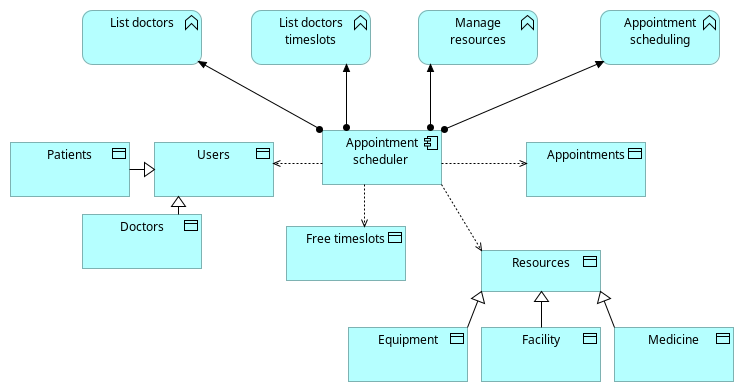
\includegraphics[width=\textwidth]{./fig/5. Application Monolith.png}
    \caption{Application architecture pt. 1: A monolithic backend}
    \label{fig:monolith}
\end{figure}

\subsection{Microservices}

Figure~\ref{fig:microservices} represents the second implementation and
illustrates the flow of interactions between the "Web app", an "API Gateway",
and various microservices. The "API Gateway" acts as an entry
point, routing requests from the "Web app" to the appropriate microservices:
"User service", "Appointment service", and "Resources service".

\begin{figure}[H]
    \centering
    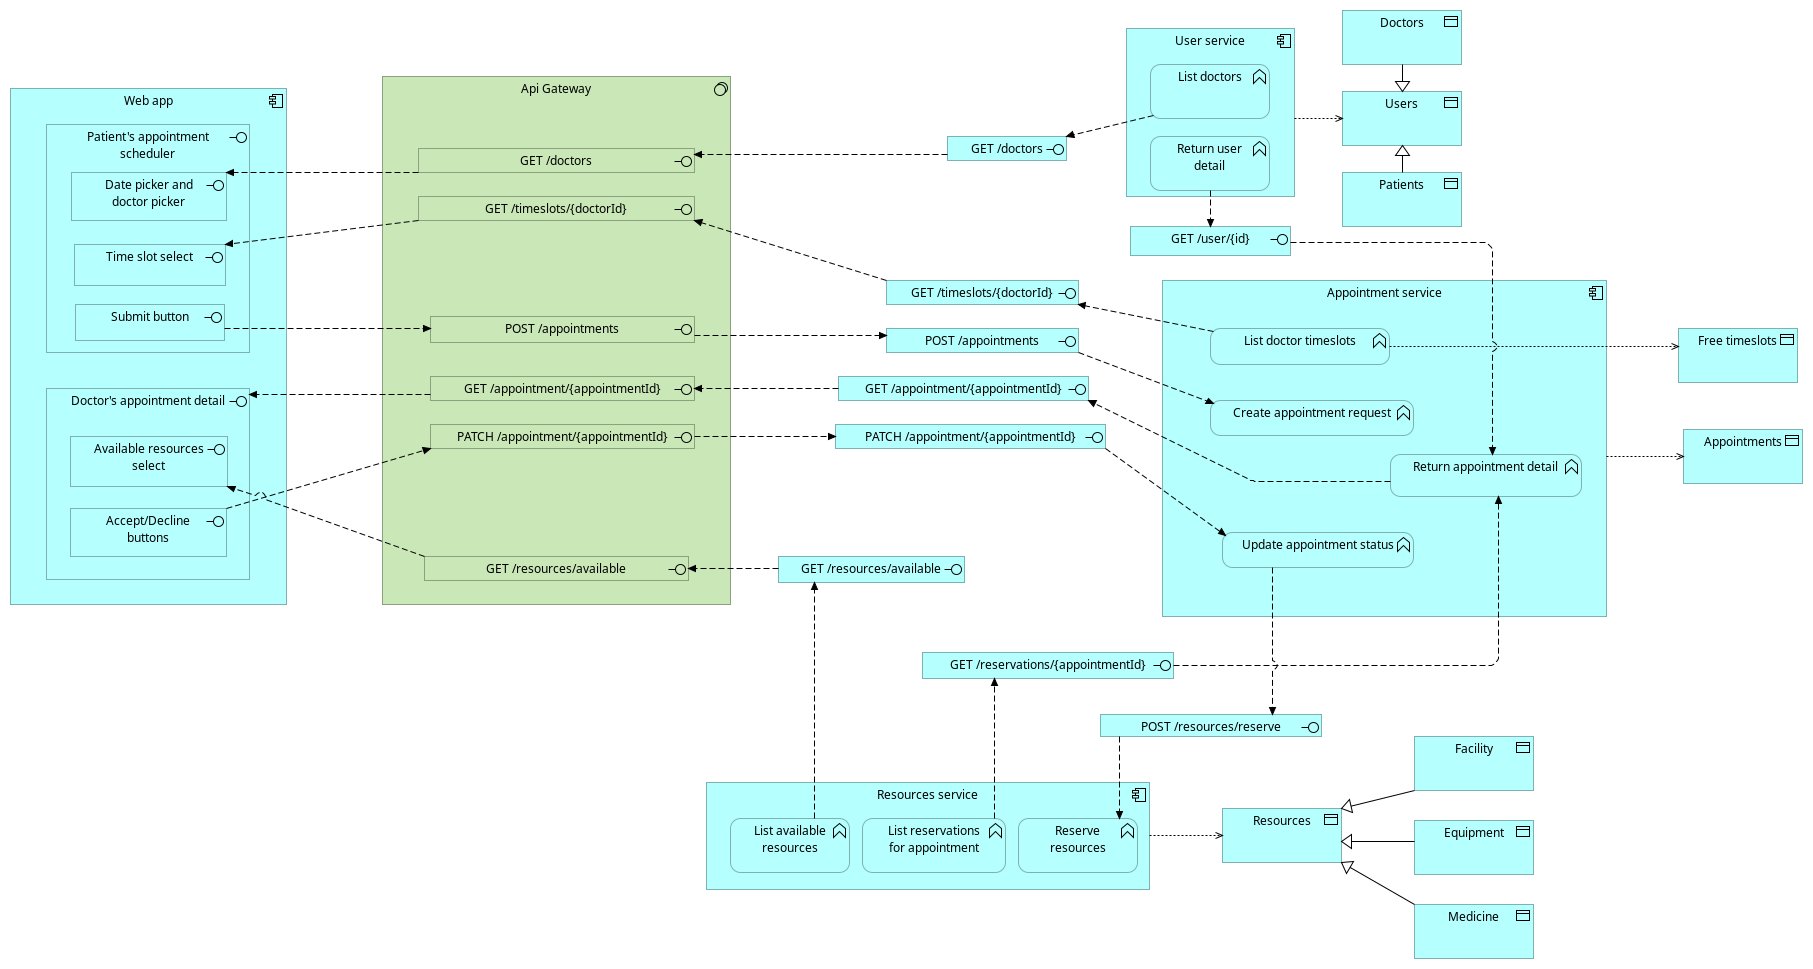
\includegraphics[width=\textwidth]{./fig/6. Application Microservices.png}
    \caption{Application architecture pt. 2: Microservices}
    \label{fig:microservices}
\end{figure}

\subsection{Camunda oriented architecture}

Figure~\ref{fig:camunda} models how the process can be supported with
the integration of Camunda, specifically showing the "Camunda Schedule
appointment process" component. This process interacts with an "External
worker service" to "Reserve resources". Since our implementation doesn't
use embedded Camunda, it can slightly resemble event driven architecture,
since Camunda emits topics, which the external worker consumes and then
submits the task results back to Camunda.

\begin{figure}[H]
    \centering
    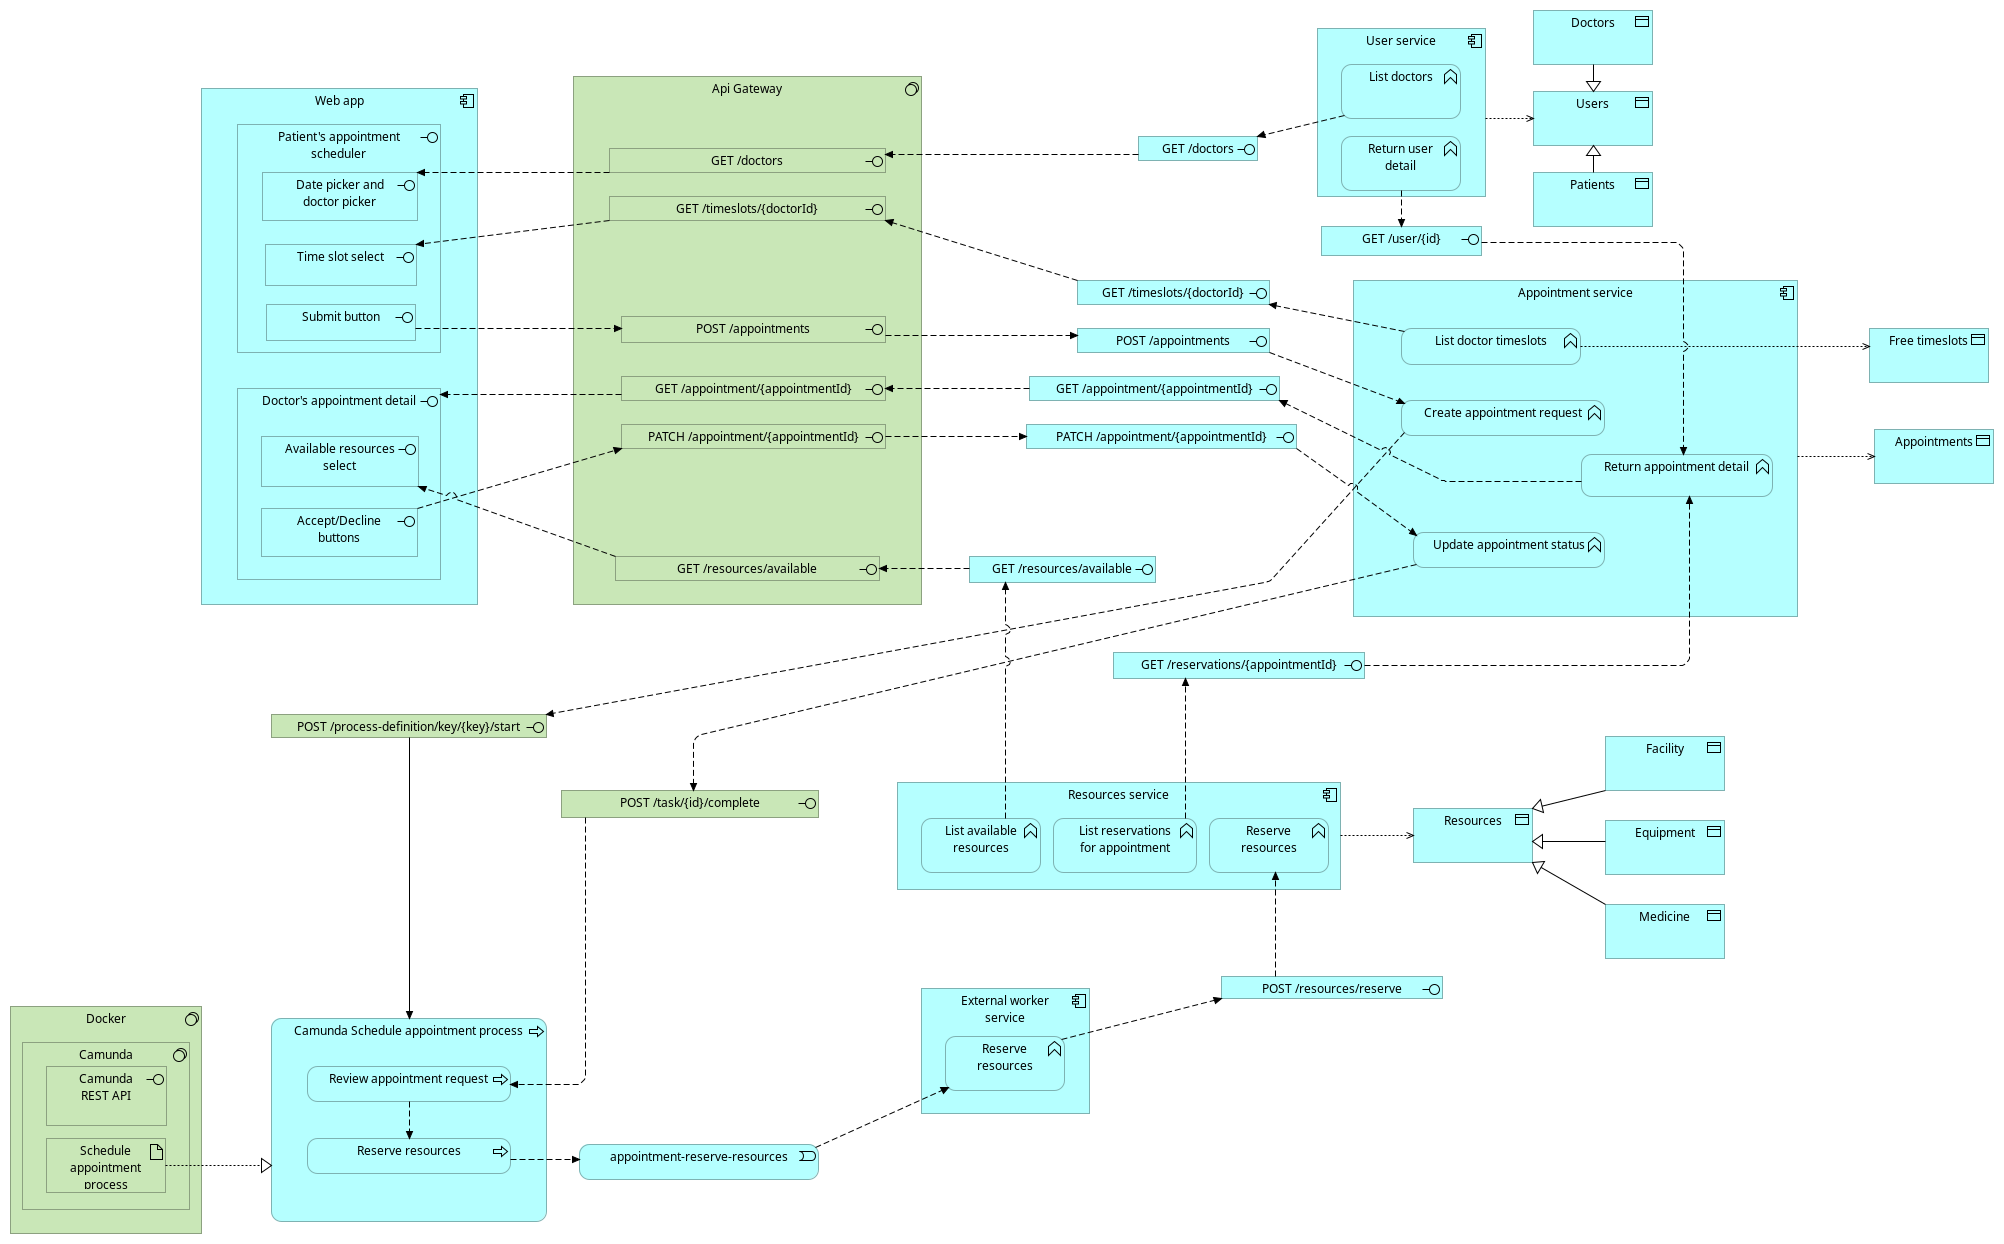
\includegraphics[width=\textwidth]{./fig/7. Application Camunda.png}
    \caption{Application architecture pt. 3: Camunda oriented architecture}
    \label{fig:camunda}
\end{figure}

Figure~\ref{fig:bpmn-appt} presents a business process model diagram
detailing the "Camunda Schedule appointment process".
The process begins with an "Appointment request". This triggers a user task,
"Review appointment request", where a decision is made. An exclusive gateway,
labeled "Decision made?", routes the flow. If the request is "Accepted", a
service task "Reserve resources" is executed, leading to the "Appointment
scheduled" end event. If "Denied", the process directly reaches the
"Appointment denied" end event.

\begin{figure}[H]
    \centering
    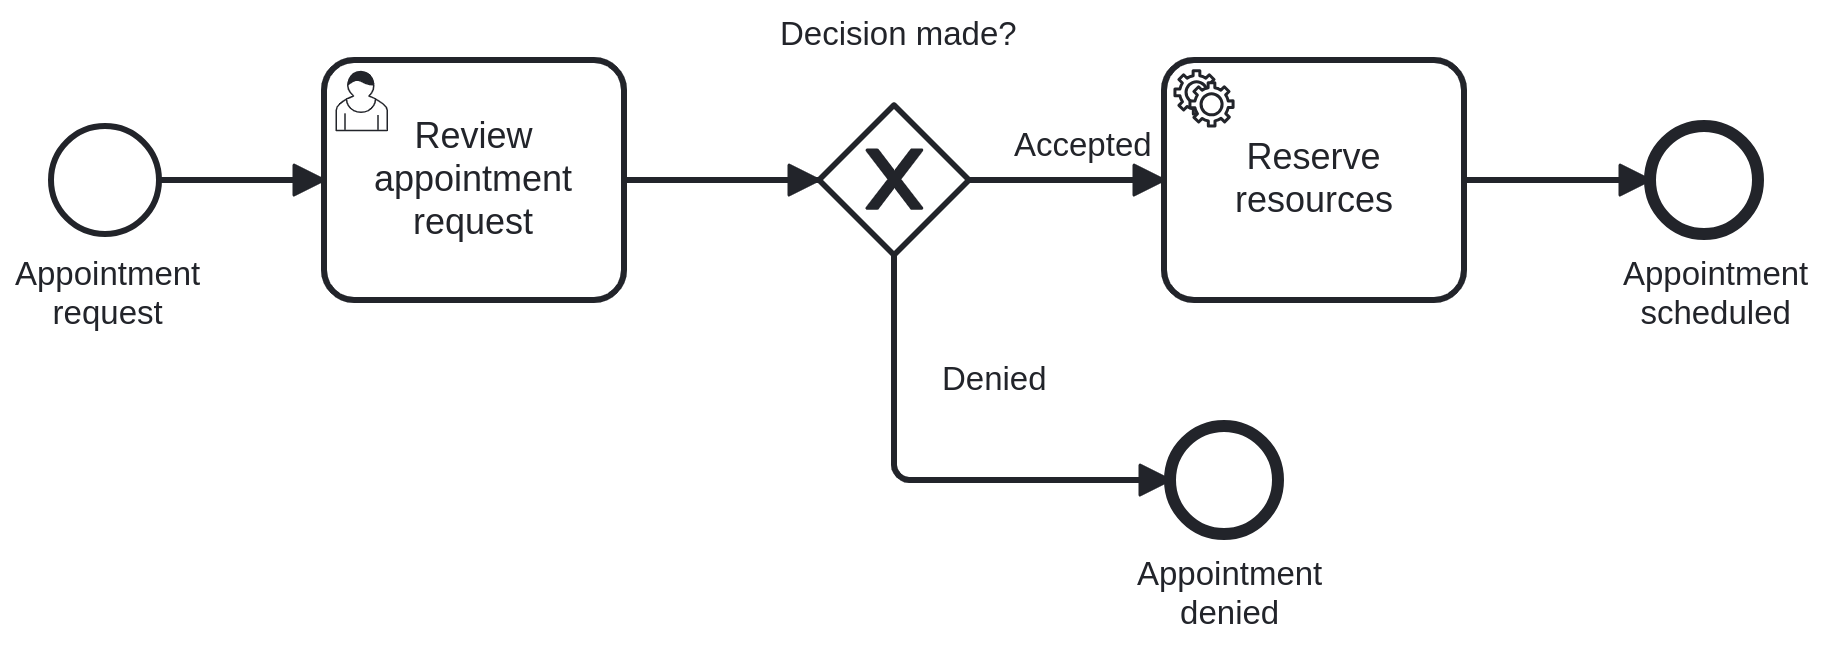
\includegraphics[width=\textwidth]{./fig/bpmn-appt-scheduling.png}
    \caption{Schedule appointment process BPMN}
    \label{fig:bpmn-appt}
\end{figure}

\subsection{Event driven architecture with Kafka}

Figure~\ref{fig:kafka} details the usage of Kafka for asynchronous
communication within the system. Kafka is run in a Docker container,
which includes a "Kafka Custom TCP listener" endpoint. The "Appointment service"
publishes "Appointment status update" messages to Kafka, and the "Resources
service" consumes these messages and publishes "Resource reserved"
messages.

\begin{figure}[H]
    \centering
    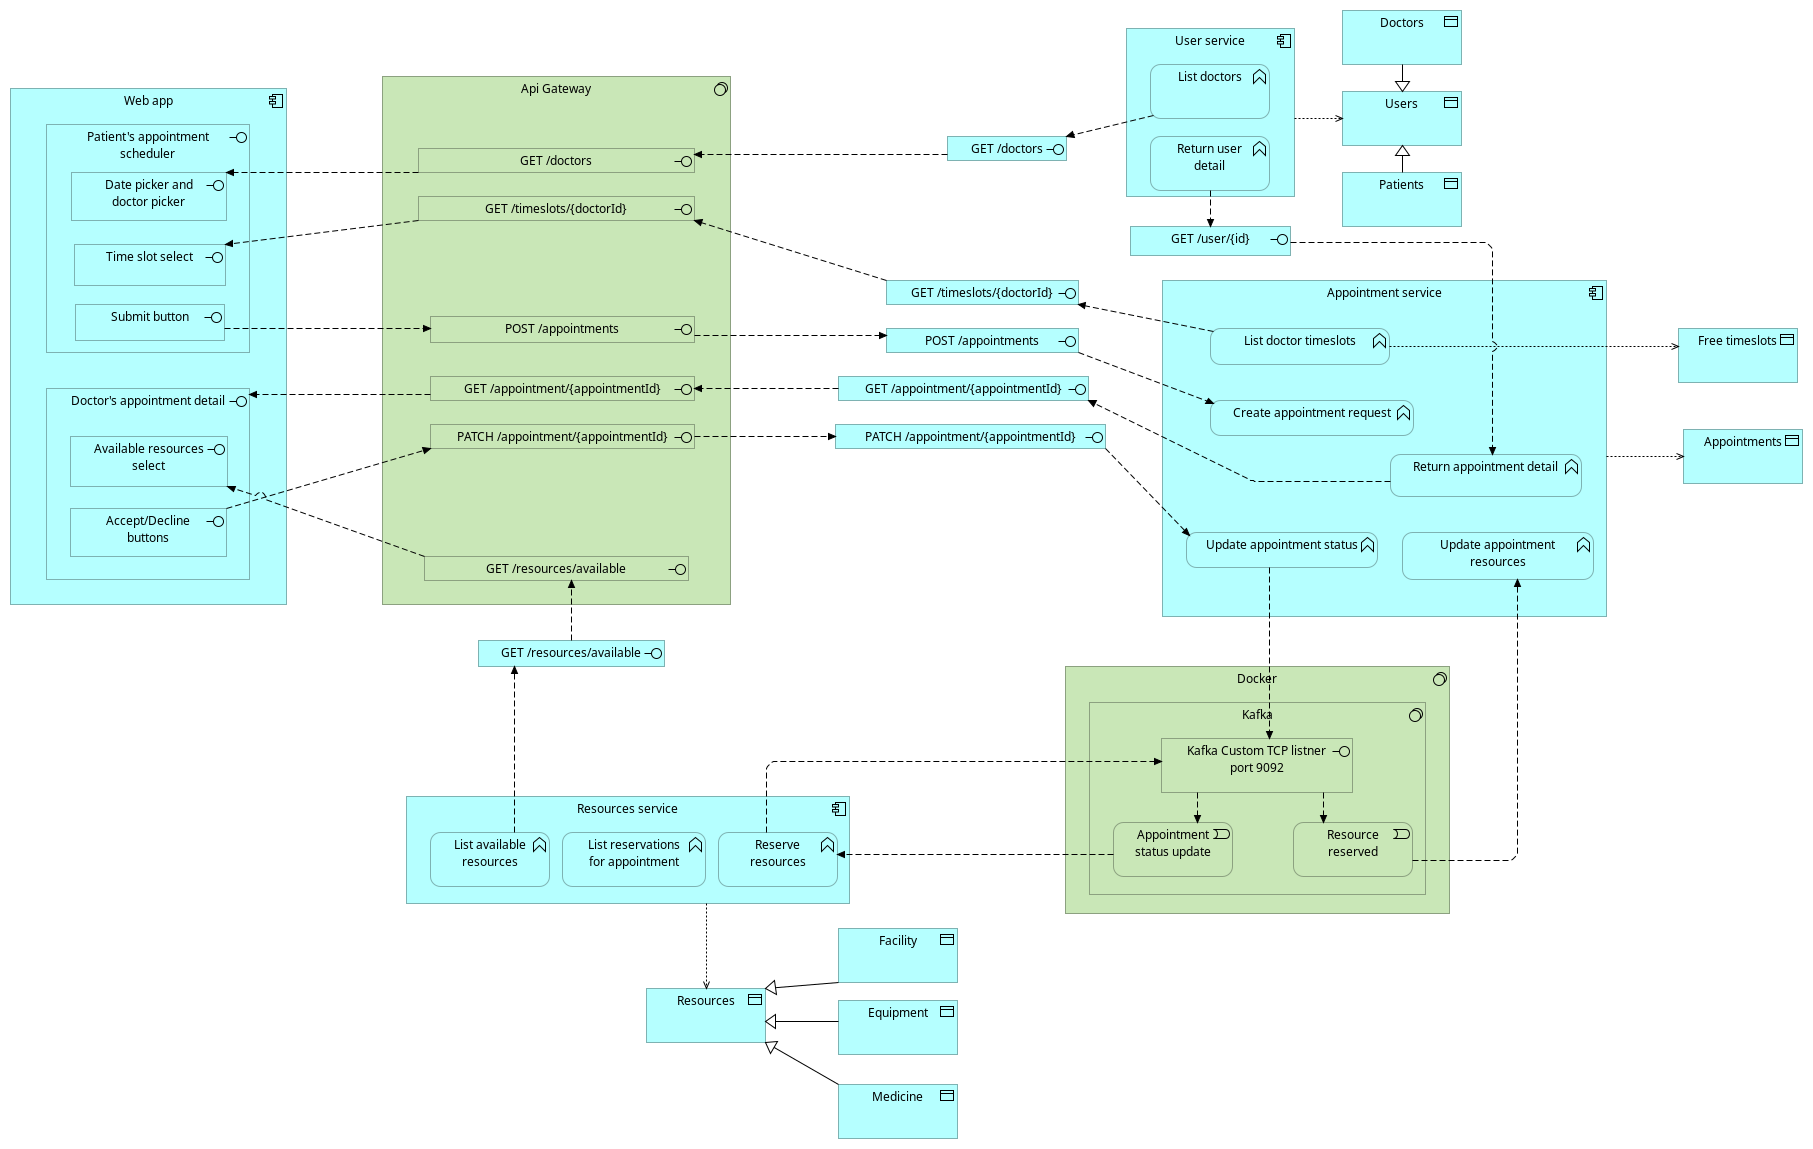
\includegraphics[width=\textwidth]{./fig/8. Application Kafka.png}
    \caption{Event driven architecture with Kafka}
    \label{fig:kafka}
\end{figure}

\section{Conclusion}

We successfully developed a simple medical calendar application in 4
different architectures, focusing on the core "Schedule an appointment"
process.

We explored various architectural approaches for the backend.
Implementing and modeling monolithic, microservices, Camunda oriented, and
event-driven architectures using Kafka, without requiring frontend implementation
to change.

\end{document}
